\section{Experiments} \label{sec:exp}

A prototype version of {\FORPI} has been implemented in the functional programming language Scala as part of the \skeptik
library. This library includes an implementation of {\GFOLU} \cite{GFOLU}. 
Note that by implementing the algorithms in this library, we have a relative guarantee that the compressed proofs are correct, as in \skeptik every inference rule (e.g. resolution, factoring) is implemented as a small class (each at most 178 lines of code that is assumed correct) with a constructor that checks whether the conditions for the application of the rule are met, thereby preventing the creation of objects representing incorrect proof nodes (i.e. unsound inferences). We only need to check that the root clause of the compressed proof is equal to or stronger than the root clause of the input proof and that the set of axioms used in the compressed proof is a subset of the set of axioms used in the input proof.


{\FORPI} was evaluated on the same 308 proofs generated by {\SPASS} to evaluate {\GFOLU}, as well as 2280 (the same number of problems initially given to {\SPASS}) randomly generated proofs. Proof lengths varied from 3 to 700, while the number of resolutions in a proof ranged from 1 to 368 (1-32 resolutions for proofs in the TPTP data set; 1-368 resolutions for the proofs in the random data set). The same laptop was used to perform proof compression. Details and a discussion regarding the realism reflected in the random proofs are in the next subsection.
The proofs are available at \url{https://github.com/jgorzny/Skeptik}.

%\subsection{Proof Generation}
Additional proofs were generated by the following procedure: start with a root node whose conclusion is $\bot$, and make two premises $\eta_1$ and $\eta_2$ using a randomly generated literal such that the desired conclusion is the result of resolving $\eta_1$ and $\eta_2$. For each node $\eta_i$, determine the inference rule used to make its conclusion: with probability $p=0.9$, $\eta_i$ is the result of a resolution, otherwise it is the result of  factoring. 

Literals are generated by uniformly choosing a number from $\{1,\dots,k,k+1\}$ where $k$ is the number of predicates generated so far; if the chosen number $j$ is between $1$ and $k$, the $j$-th predicate is used; otherwise, if the chosen number is $k+1$, a new predicate with a new random arity (at most four) is generated and used. Each argument is a constant with probability $p=0.7$ and a complex term (i.e. a function applied to other terms) otherwise; functions are generated similarly to predicates. 

If a node $\eta$ should be the result of a resolution, then with probability $p=0.2$ we generate a left parent $\eta_\ell$ and a right parent $\eta_r$ for $\eta$ (i.e. $\eta = \eta_\ell \odot \eta_r$) having a common parent $\eta_c$ (i.e. $\eta_l = (\eta_\ell)_\ell \odot \eta_c$ and $\eta_r = \eta_c \odot (\eta_r)_r$, for some newly generated nodes $(\eta_\ell)_\ell$ and $(\eta_r)_r$ ). The common parent ensures that also non-tree-like DAG proofs are generated. 

This procedure is recursively applied to the generated parent nodes. 
Each parent of a resolution has each of its terms not contained in the pivot replaced by a fresh variable with probability $p=0.7$.
At each recursive call, the additional minimum height required for the remainder of the branch is decreased by one with probability $p=0.5$. Thus if each branch always decreases the additional required height, the proof has height equal to the initial minimum value. The process stops when every branch is required to add a subproof of height zero or after a timeout is reached. In any case, the topmost generated node for each branch is generated as an axiom node. 

The minimum height was set to 7 (which is the minimum number of nodes in an irregular proof plus one) and the timeout was set to 300 seconds (the same timeout allowed for {\SPASS}). The probability values used in the random generation were carefully chosen to produce random proofs similar in shape to the real proofs obtained by {\SPASS}. For instance, the probability of a new node being a resolution (respectively, factoring) is approximately the same as the frequency of resolutions (respectively, factorings) observed in the real proofs produced by {\SPASS}.



\subsection{Results}

For each proof $\psi$, we measured the time needed to compress the proof ($t(\psi)$) and the compression ratio ($(|\psi|-|\alpha(\psi)|)/|\psi|$) where $|\psi|$ is the number of resolutions in the proof, and $\alpha(\psi)$ is the result of applying a compression algorithm or some composition of {\FORPI} and {\GFOLU}. Note that we consider only the number of resolutions in order to compare the results of these algorithms to their propositional variants (where factoring is implicit). Moreover, factoring could be made implicit within resolution inferences even in the first-order case and we use explicit factoring only for technical convenience.





\begin{table*}[bt]
\centering
\begin{scriptsize}
%\hspace*{-0.5cm}
\begin{tabular}{| l | r | r | r | r | r | r  | }
\hline
 Algorithm& \multicolumn{3}{c |}{\# of Proofs Compressed} & \multicolumn{3}{c |}{\# of Removed Nodes}  \\
& \multicolumn{1}{c }{TPTP} & \multicolumn{1}{c}{Random}  & \multicolumn{1}{c |}{Both}  & \multicolumn{1}{c }{TPTP} & \multicolumn{1}{c }{Random} & \multicolumn{1}{c |}{Both}  \\ \hline 
{\GFOLU}(p) & 55 (17.9\%) & 817 (35.9\%) & 872 (33.7\%)  & 107 (4.8\%) & 17,769 (4.5\%) & 17,876 (4.5\%)    \\ \hline
{\FORPI}(p)  & 23 (7.5\%) &  666 (29.2\%) & 689 (26.2\%)  &  36 (1.6\%) &  28,904 (7.3\%) &  28,940 (7.3\%)   \\ \hline
{\GFOLU}({\FORPI}(p))   & 55 (17.9\%) & 1303 (57.1\%) & 1358 (52.5\%) & 120 (5.4\%)  & 48,126 (12.2\%) & 48,246 (12.2\%) \\ \hline
{\FORPI}({\GFOLU}(p)) & 23 (7.5\%) & 1302  (57.1\%)&  1325 (51.2\%) & 120 (5.4\%) & 48,434 (12.3\%) & 48,554 (12.3\%)  \\ \hline
Best                            & 59 (19.2\%) & 1303 (57.1\%) & 1362 (52.5\%)   & 120 (5.4\%) & 55,530 (14.1\%) & 55,650 (14.0\%)     \\ \hline
\end{tabular} $~~~~~~~~~~~~~~~~$
\end{scriptsize}
%\vspace{3pt}
\caption{Number of proofs compressed and number of overall nodes removed.}
\label{tab:results}
\end{table*}




\begin{table*}[bt]
\centering
\begin{scriptsize}
\begin{tabular}{| l | r | r | l | r |}
\hline
Algorithm &  \multicolumn{2}{c |}{First-Order Compression}  &  Algorithm & Propositional Compression \cite{Boudou}  \\
& $~~~~$ All   & Compressed Only & & \\ \hline
{\GFOLU}(p) &  4.5\%& 13.5\% &{\LU}(p) & 7.5\% \\ \hline
{\FORPI}(p) & 6.2\%&  23.2\%&{\RPI}(p) &  17.8\% \\ \hline
{\GFOLU}({\FORPI}(p)) &  10.6\%& 23.0\%& ({\LU}({\RPI}(p)) &  21.7\% \\ \hline
{\FORPI}({\GFOLU}(p)) &  11.1\%& 21.5\%& ({\RPI}({\LU}(p)) & 22.0\% \\ \hline
Best & 12.6\% & 24.4\%&  Best &  22.0\% \\ \hline
\end{tabular}
\end{scriptsize}
%\vspace{3pt}
\caption{Mean compression results.}
\label{tab:result-mean}
\end{table*}

Table \ref{tab:results} summarizes the results of {\FORPI} and its combinations with {\GFOLU}. The first set of columns describes the percentage of proofs that were compressed by each compression algorithm. The algorithm `Best' runs both combinations of {\GFOLU} and {\FORPI} and returns the shortest proof output by either of them. The total number of proofs is $308+2280=2588$ and the total number of resolution nodes is $2,249 + 393,883
= 396,132$. The percentages in the last three columns are computed by $(\Sigma_{\psi \in \Psi} |\psi|  - \Sigma_{\psi\in \Psi} |\alpha(\psi)|)/(\Sigma_{\psi \in \Psi} |\psi|)$ for each data set $\Psi$ (TPTP, Random, or Both: the union of the other two data sets). 
The use of both algorithms allows at least an additional 17.5\% of proofs to be compressed. Furthermore, the use of both algorithms removes almost twice as many nodes than any single algorithm.
Only nine proofs from the TPTP data set were compressed by {\FORPI}, reducing the number of resolutions by at least one and at most three. Given the size of the TPTP proofs, it is unsurprising that few are compressed: small proofs are a priori less likely to contain irregularities. However, 252 (0.11\%) of the randomly generated proofs achieved some compression using only {\FORPI}. 

Table \ref{tab:result-mean} compares the results of {\FORPI} and its combinations with {\GFOLU} (on first-order proofs) with their propositional variants (on propositional proofs) as evaluated in \cite{Boudou}. The first column describes the mean compression ratio for each algorithm including proofs that were not compressed by the algorithm, while the second column calculates the mean compression ratio considering only compressed proofs. It is unsurprising that the first column is lower than the propositional mean for each algorithm: there are stricter requirements to apply these algorithms to first-order proofs. In particular, additional properties must be satisfied before a unit can be lowered, or before a pivot can be recycled. On the other hand, when first-order proofs are compressed, the compression ratios of the first-order algorithms are on par with or better than their propositional counterparts.

\newcommand{\csubfloat}[2][]{%
  \makebox[0pt]{\subfloat[#1]{#2}}%
}
\newcommand{\centerhfill}[1][\quad]{\hspace{\stretch{0.5}}#1\hspace{\stretch{0.5}}}
%
\newcommand{\csubfloat}[2][]{%
  \makebox[0pt]{\subfloat[#1]{#2}}%
}
\newcommand{\centerhfill}[1][\quad]{\hspace{\stretch{0.5}}#1\hspace{\stretch{0.5}}}

\begin{figure*}[bt]
\hspace{-1cm}
\begin{centering}
\makebox[\textwidth]{\makebox[1.25\textwidth]{
\begin{minipage}{0.3\textwidth}\centering
\subfloat[Compressed length against input length]{{
    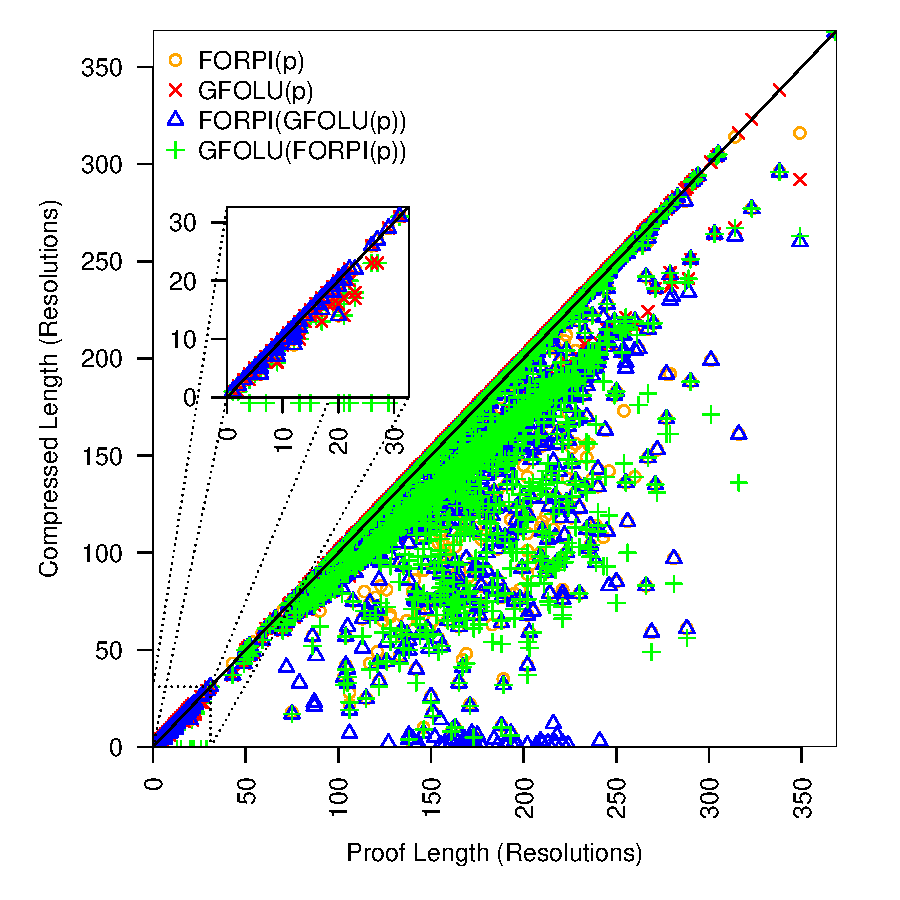
\includegraphics[scale=0.4]{images-new/combined-all-res-length-vs-compressed-res-length.pdf}%
    }}
 \end{minipage}\hfill
\begin{minipage}{0.3\textwidth}\centering
\subfloat[\FORPI(\GFOLU(p)) vs. \GFOLU(\FORPI(p))]{{
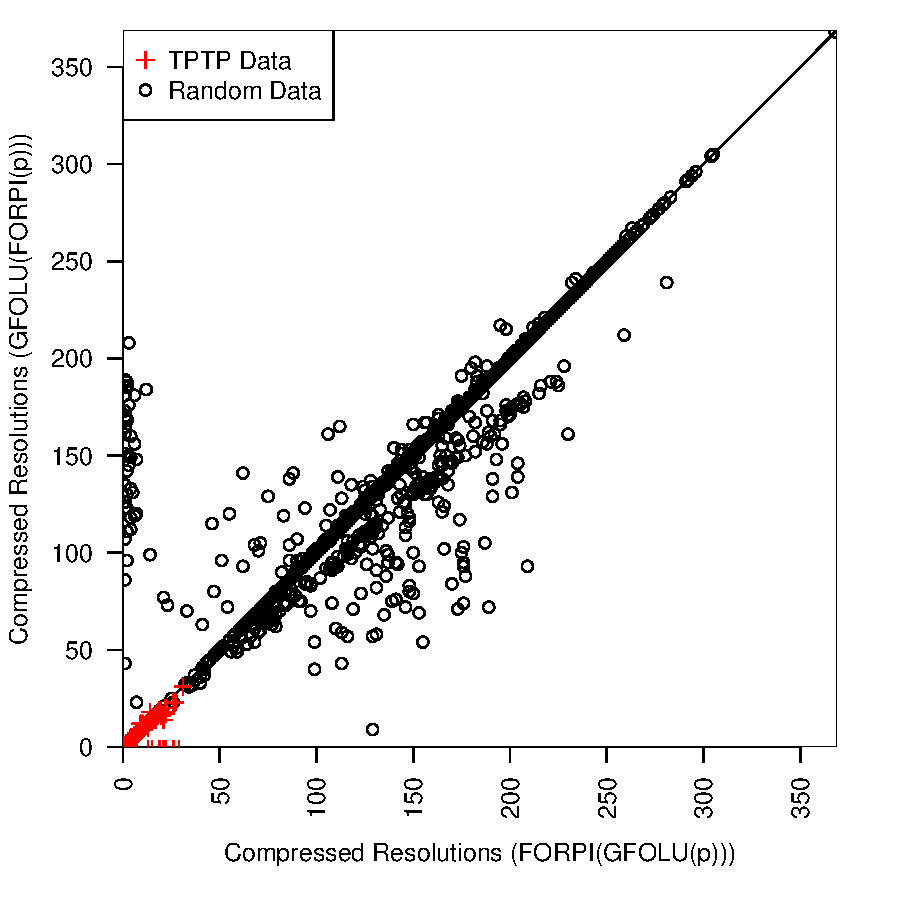
\includegraphics[scale=0.4]{images-new/combined-alg-res.pdf}%
}}
 \end{minipage}\hfill
\begin{minipage}{0.3\textwidth}\centering
\subfloat[Cumulative proof compression]{{
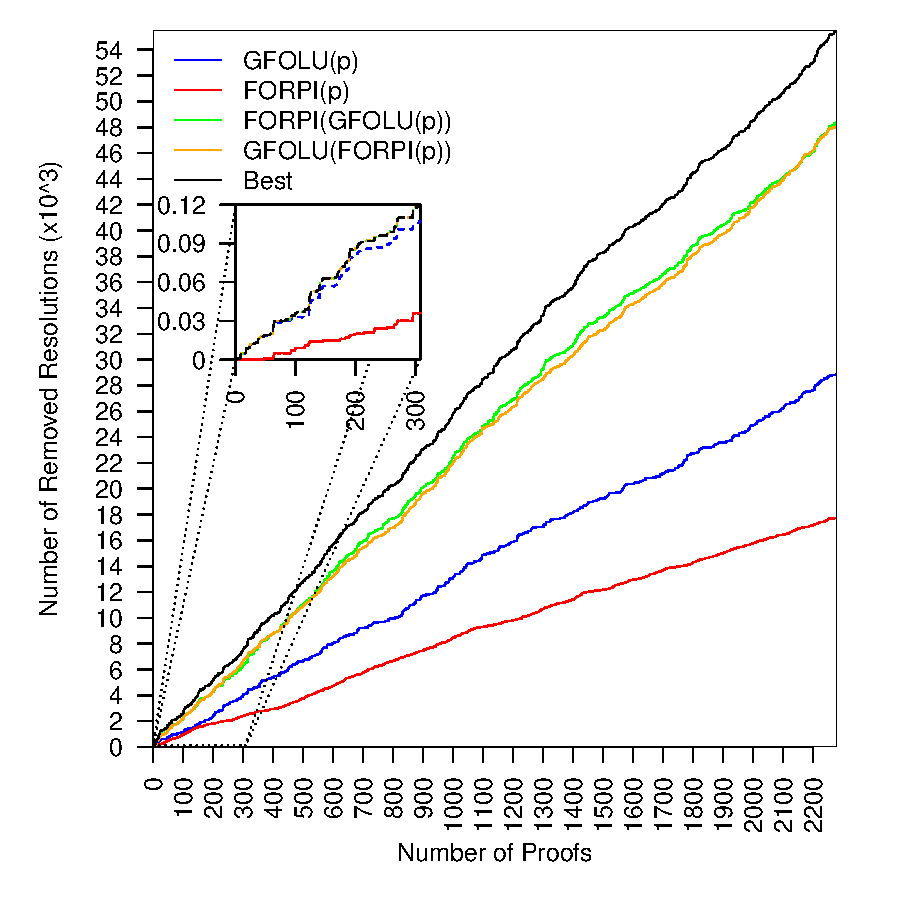
\includegraphics[scale=0.4]{images-new/combined-all-cumulative-res-nodes-diff.pdf}%
}}
 \end{minipage}
 }}\end{centering}
 \caption{\GFOLU \& \FORPI Combination Results}
\label{fig:ex}
\end{figure*}
 %Turn off two commands above before putting this in
\begin{figure*}[bt]
\centering
%\hspace{-1cm}
%\begin{centering}
%\makebox[\textwidth]{\makebox[1.25\textwidth]{
%\begin{minipage}{0.3\textwidth}\centering
\subfloat[Compressed length against input length.]{{
    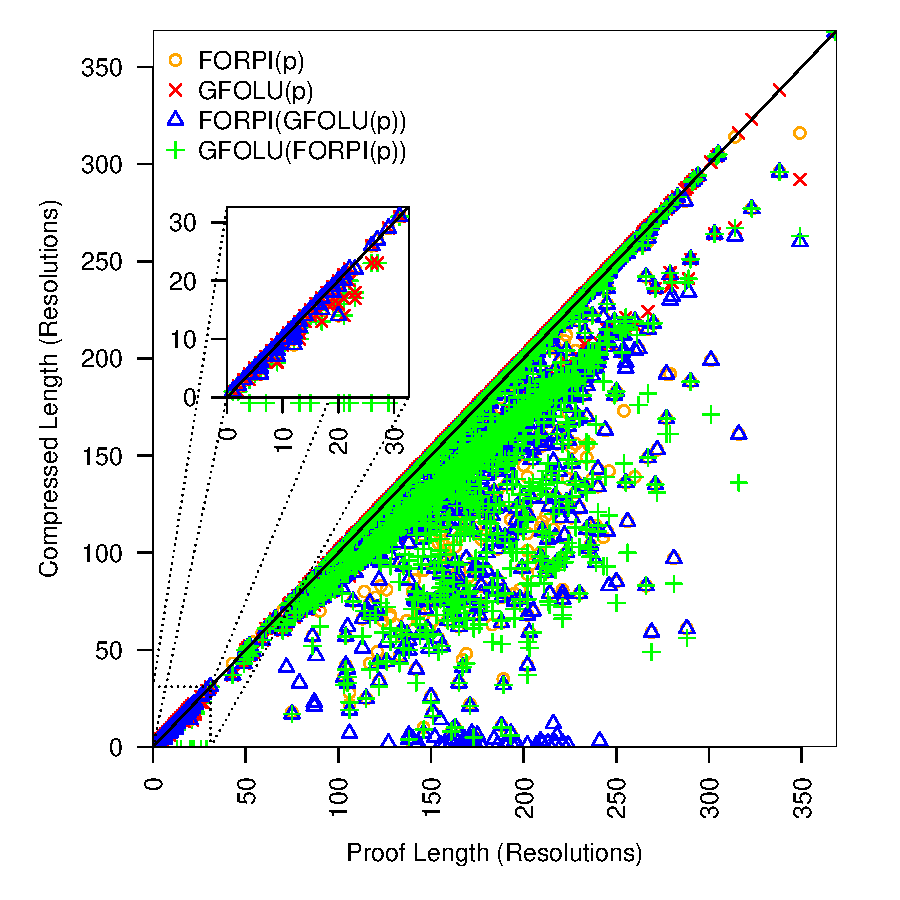
\includegraphics[scale=0.35]{images-new/combined-all-res-length-vs-compressed-res-length.pdf}%
    }}
% \end{minipage}\hfill
%\begin{minipage}{0.3\textwidth}\centering
\subfloat[\FORPI(\GFOLU(p)) vs. \GFOLU(\FORPI(p)).]{{
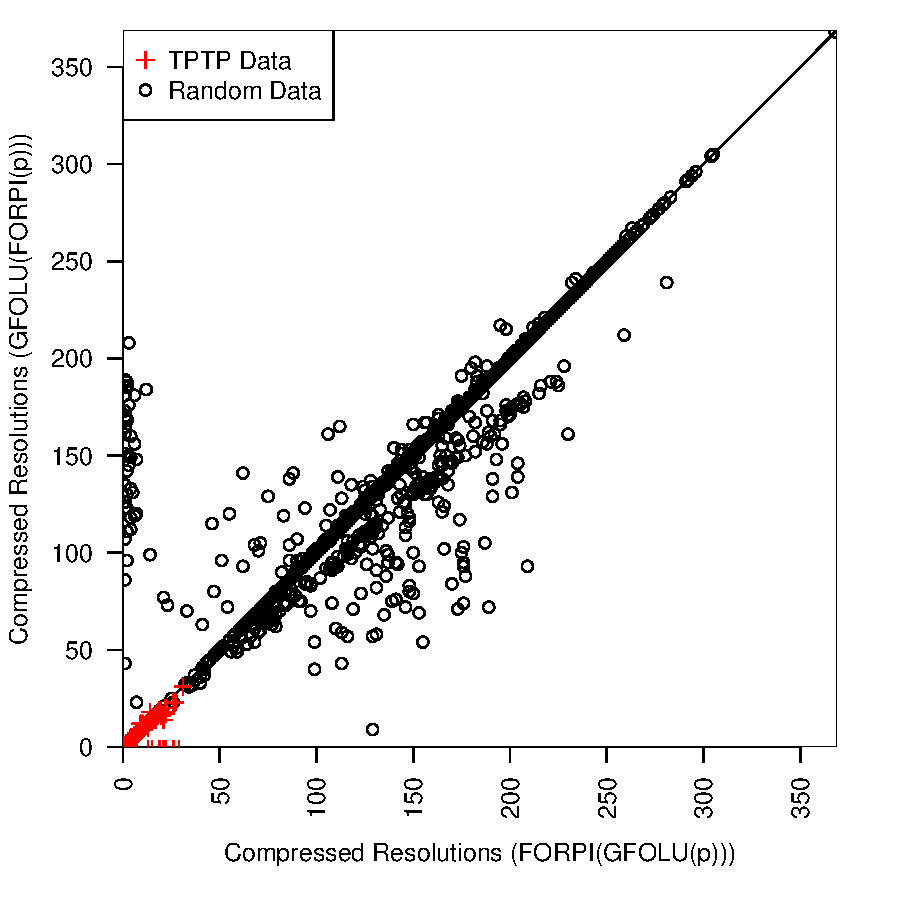
\includegraphics[scale=0.35]{images-new/combined-alg-res.pdf}%
}}\\
 %\end{minipage}\hfill
%\begin{minipage}{0.3\textwidth}\centering
\subfloat[Cumulative proof compression.]{{
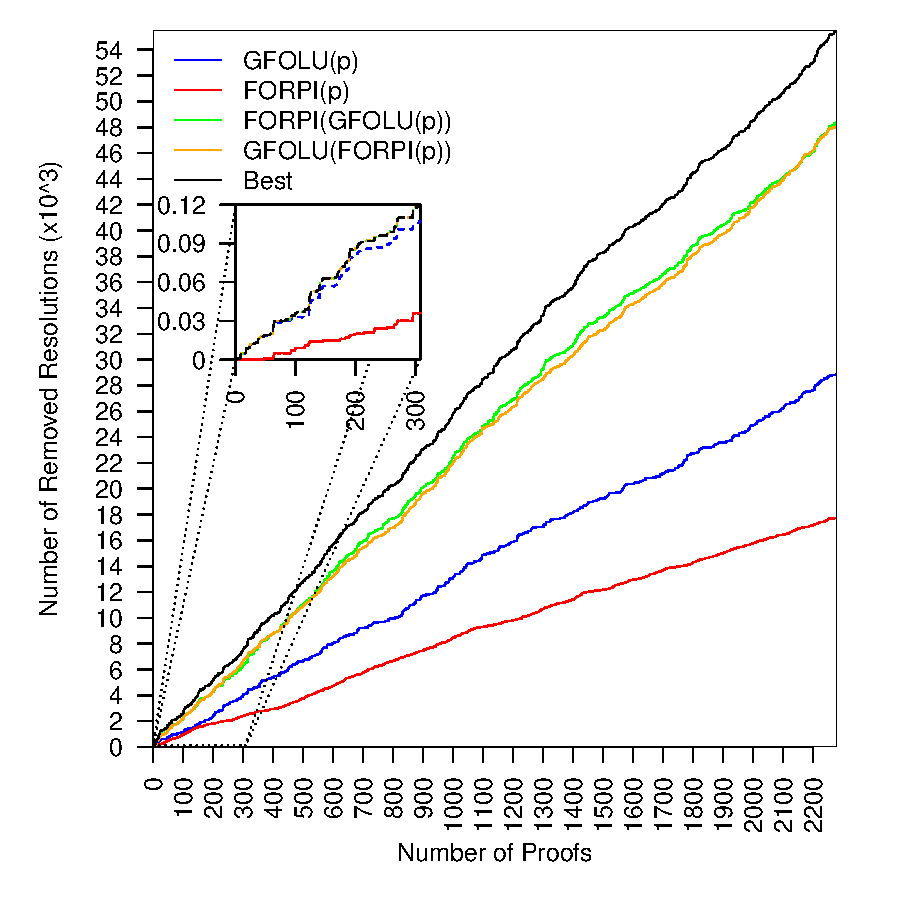
\includegraphics[scale=0.35]{images-new/combined-all-cumulative-res-nodes-diff.pdf}%
}}
% \end{minipage}
% }
 %}
 %\end{centering}
 \caption{\GFOLU \& \FORPI Combination Results.}
\label{fig:ex}
\end{figure*}





Figure \ref{fig:ex} (a) is a scatter plot comparing the number of resolutions of the input proof against the number of resolutions in the compressed proof for each algorithm. The results on the TPTP data are magnified in the sub-plot. For the randomly generated proofs (points outside of the sub-plot), it is often the case that the compressed proof is significantly shorter than the input proof. Interestingly, {\GFOLU} appears to reduce the number of resolutions by a linear factor in many cases. This is likely due to a linear growth in the number of non-interacting irregularities (i.e. irregularities for which the lowered units share no common literals with any other sub-proofs), which leads to a linear number of nodes removed.



Figure \ref{fig:ex} (b) is a scatter plot comparing the size of compression obtained by applying {\FORPI} before {\GFOLU} versus {\GFOLU} before {\FORPI}. Data obtained from the TPTP data set is marked in red; the remaining points are obtained from randomly generated proofs. Points that lie on the diagonal line have the same size after each combination. There are 249 points beneath the line and 326 points above the line. Therefore, as in the propositional case \cite{LURPI}, it is not a priori clear which combination will compress a proof more. 
Applying {\FORPI} after {\GFOLU} is more likely to maximize the likelihood of compression, and the achieved compression also tends to be larger.

Figure \ref{fig:ex} (c) shows a plot comparing the difference between the cumulative number of resolutions of the first $x$ input proofs and the cumulative number of resolutions in the first $x$ proofs after compression (i.e. the cumulative number of \emph{removed} resolutions). The TPTP data is displayed in the sub-plot; note that the lines for everything except {\FORPI} largely overlap (since the values are almost identical; cf. Table \ref{tab:results}). The data shows that the best approach is to try both combinations of {\FORPI} and {\GFOLU} and choose the best result.


Proof generation required approximately 110 minutes (including some cluster time), while the total time to apply both algorithms on all these proofs was just over 7.5 minutes, only 6.8\% more time than generating proofs in the first place, on a simple laptop computer. All times include parsing time.  These compression algorithms are still fast in the first-order case, and may simplify the proof considerably for a relatively small cost in time.



The use of {\FORPI} alongside {\GFOLU} allows at least an additional 17.5\% of proofs to be compressed. Furthermore, the likelihood of compression is maximized by applying {\FORPI} after {\GFOLU}, and trying both compositions may be even more beneficial. 
On large proofs, thousands of nodes may be removed quickly relative to the time required to initially generate the proof.



